\chapter{Colour and Absorbance}\label{ch:g11:absorbance}

A bottle of sports drink glows bright blue on the bench of a gym. Its
colour comes from a dye dissolved in it, a few milligrams in a whole
litre: far too little to weigh, and far too little to see as a solid.
Yet a food laboratory must check that amount, because a dye may be added
only within limits. The colour itself is the key. The more dye a
solution holds, the more light it absorbs; an instrument that measures
how much light a solution absorbs measures, in fact, a concentration.

\begin{recall}
The mass and \omterm{def:g10:concentration-and-dilution:molar-concentration}{molar concentrations} of a solution; diluting a \omterm{def:g10:concentration-and-dilution:dilution}{stock
solution}; a \omterm{def:g10:concentration-and-dilution:standard}{calibration scale} of \omterm{def:g10:concentration-and-dilution:standard}{standard solutions} compared with an
unknown (\cref{ch:g10:concentration-and-dilution}).
\end{recall}

\begin{omfigure}
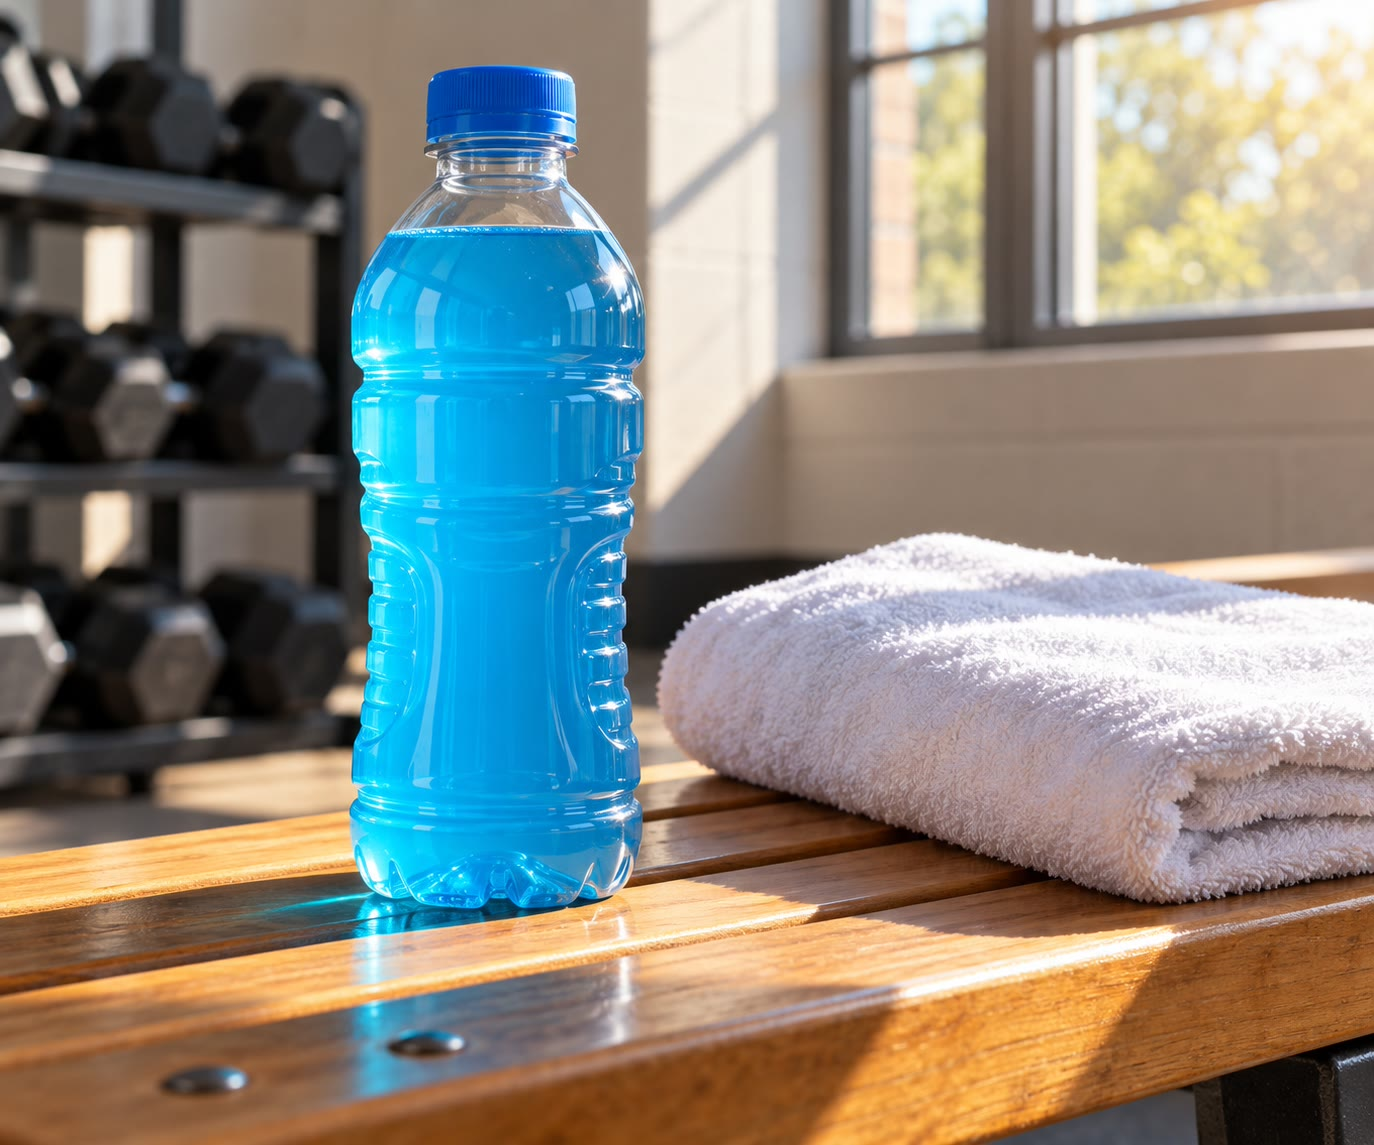
\includegraphics[width=0.5\linewidth]{images/book1/ai/g11-sports-drink.jpg}

{\small A blue drink: its colour comes from a few milligrams of dye per
litre.}
\end{omfigure}

\section{The colour of a solution}

White light, such as daylight, is a \omterm{def:g6:pure-substances-and-mixtures:mixture}{mixture} of all the colours of the
rainbow. Each colour corresponds to a wavelength, from about
\qty{400}{nm} for violet to about \qty{750}{nm} for red; the physics
book explains what a wavelength is, and here it is only a label for a
colour. A coloured solution absorbs part of the light that crosses it,
some colours much more than others; the eye sees the colours that pass
through.

\begin{definition}[Complementary colours]\label{def:g11:absorbance:complementary}
Two colours are \emph{complementary colours}\index{complementary colours}
if mixing them gives white light. On a colour wheel, complementary
colours face each other.
\end{definition}

\begin{omfigure}
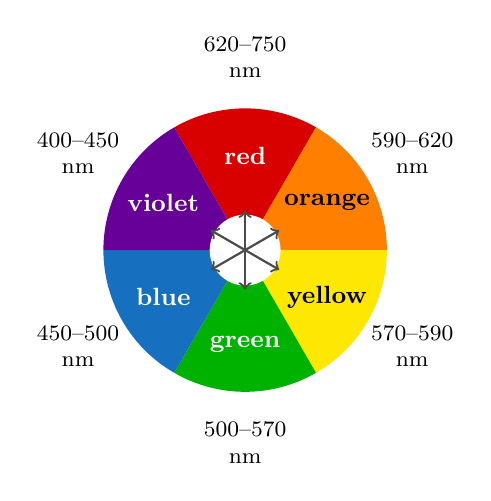
\begin{tikzpicture}[font=\small]
  \foreach \a/\c/\n/\w/\t in {90/red!85!black/red/{620--750}/white,
      30/orange/orange/{590--620}/black, -30/yellow!90!orange/yellow/{570--590}/black,
      -90/green!70!black/green/{500--570}/white, -150/cyan!50!blue/blue/{450--500}/white,
      150/violet!80!blue/violet/{400--450}/white} {
    \fill[\c] (0,0) -- (\a-30:1.8) arc[start angle=\a-30, end angle=\a+30,
      radius=1.8] -- cycle;
    \node[text=\t, font=\small\bfseries] at (\a:1.2) {\n};
    \node[font=\footnotesize, align=center] at (\a:2.45) {\w\\ nm};
  }
  \fill[white] (0,0) circle (0.45);
  \draw[<->, thick, black!70] (90:0.5) -- (-90:0.5);
  \draw[<->, thick, black!70] (30:0.5) -- (-150:0.5);
  \draw[<->, thick, black!70] (-30:0.5) -- (150:0.5);
\end{tikzpicture}

{\small A colour wheel, with approximate wavelengths. \omterm{def:g11:absorbance:complementary}{Complementary
colours} face each other: red and green, orange and blue, yellow and
violet.}
\end{omfigure}

\begin{proposition}[The colour seen]\label{prop:g11:absorbance:colour-seen}
A solution that absorbs mainly one colour of white light looks the
colour complementary to it.
\end{proposition}

\begin{proof}
Admitted: the light that passes is white light minus the absorbed
colour, and the eye sees that remainder as the complementary colour.
\end{proof}

\begin{example}[Two food dyes]\label{ex:g11:absorbance:dyes}
% ledger: lmax:E133, lmax:E102
The blue dye of the sports drink, known as Brilliant Blue (E133),
absorbs mostly orange-red light, around \qty{629}{nm}: it looks blue. The
yellow dye tartrazine (E102) absorbs mostly violet-blue light, around
\qty{427}{nm}: it looks yellow. A green drink usually holds both.
\end{example}

\section{The absorption spectrum}

\begin{definition}[Absorption spectrum]\label{def:g11:absorbance:spectrum}
The \emph{absorption spectrum}\index{absorption spectrum} of a solution
is the graph of the light it absorbs (its \omterm{def:g11:absorbance:absorbance}{absorbance}, defined in the next
section) against the wavelength. The wavelength at which the absorption
is largest is written $\lambda_{\max}$.
\end{definition}

\begin{omfigure}
\begin{tikzpicture}
\begin{axis}[width=0.85\linewidth, height=6cm, xmin=380, xmax=750,
    ymin=0, ymax=0.95, xlabel={wavelength $\lambda$ (\si{nm})},
    ylabel={absorbance $A$}, axis lines*=left, ymajorgrids,
    grid style={gray!20}, tick label style={font=\small},
    label style={font=\small}, xtick={400,450,500,550,600,650,700,750},
    ]
  % ledger: lmax:E133, abs:E133, lmax:E102, abs:E102 (band shapes synthetic)
  \addplot[very thick, cyan!60!blue] table[x=lambda, y=E133]
    {figdata/out/grade-11-absorbance-a.dat};
  \addplot[very thick, orange!85!yellow] table[x=lambda, y=E102]
    {figdata/out/grade-11-absorbance-a.dat};
  \node[font=\small, align=left, anchor=west, text=cyan!60!blue!80!black]
    at (axis cs:668,0.62) {blue dye E133,\\ \qty{5.0}{mg/L}};
  \node[font=\small, align=left, anchor=west, text=orange!80!black]
    at (axis cs:470,0.66) {yellow dye E102,\\ \qty{15}{mg/L}};
  \addplot[dashed, black!50] coordinates {(629,0) (629,0.82)};
  \addplot[dashed, black!50] coordinates {(427,0) (427,0.795)};
  \node[font=\small, anchor=south] at (axis cs:629,0.83) {\qty{629}{nm}};
  \node[font=\small, anchor=south] at (axis cs:427,0.81) {\qty{427}{nm}};
\end{axis}
\end{tikzpicture}

{\small Absorption spectra of the two dyes in water, in a cell
\qty{1}{cm} thick. The band shapes are drawn from a simple model; the
positions of the maxima and their heights are those of the
specifications of the two dyes.}
\end{omfigure}

\begin{remark}[Reading a spectrum]\label{rem:g11:absorbance:reading}
The blue dye absorbs almost nothing below \qty{520}{nm}: blue and violet
light pass, and the solution looks blue. The yellow dye absorbs almost
nothing above \qty{520}{nm}: green, yellow, orange and red light pass,
and the eye sees yellow. At \qty{629}{nm}, only the blue dye absorbs;
at \qty{427}{nm}, almost only the yellow one.
\end{remark}

\section{Absorbance and the spectrophotometer}

\begin{definition}[Absorbance]\label{def:g11:absorbance:absorbance}
The \emph{absorbance}\index{absorbance} $A$ of a solution, at a chosen
wavelength, is the number displayed by a spectrophotometer that measures
how much of the light of that wavelength the solution absorbs. It has no
unit; it is zero for the pure \omterm{def:g6:solutions-and-solubility:solute}{solvent}, and the larger the more light the
solution absorbs.
\end{definition}

\begin{omfigure}
\begin{tikzpicture}[font=\small]
  % lamp
  \shade[ball color=yellow!40] (0,0.6) circle (0.32);
  \foreach \a in {0,45,90,135,180,225,270,315} \draw[yellow!60!orange, thick] (\a:0.4) ++(0,0.6) -- ++(\a:0.18);
  \node[anchor=north] at (0,-0.25) {lamp};
  \draw[black!60, thick] (0.8,0.6) -- (1.75,0.6);
  % prism
  \fill[cyan!10, draw=black!60] (1.75,0.15) -- (2.55,0.15) -- (2.15,1.15) -- cycle;
  \node[anchor=north] at (2.15,-0.25) {prism};
  \foreach \c/\d in {violet/0.35, blue/0.22, green!70!black/0.08, yellow!90!orange/-0.06,
      orange/-0.2, red/-0.34}
    \draw[\c, thick] (2.45,0.6) -- (3.45,{0.6+\d});
  % slit
  \fill[black!70] (3.5,0.92) rectangle (3.6,1.4);
  \fill[black!70] (3.5,-0.2) rectangle (3.6,0.52);
  \node[anchor=north] at (3.55,-0.25) {slit};
  \draw[orange, very thick] (3.6,0.6) -- (4.75,0.6);
  % cuvette
  \pic (cv) at (5,0) {cuvette={0.75}{cyan!50!blue!45}};
  \node[anchor=north] at (5,-0.25) {cell};
  \draw[orange!60, thick] (5.3,0.6) -- (6.3,0.6);
  % detector and display
  \fill[black!15, draw=black!60] (6.3,0.2) rectangle (6.9,1.0);
  \node[anchor=north] at (6.6,-0.25) {detector};
  \draw[black!60] (6.9,0.6) -- (7.4,0.6);
  \fill[black!80, draw=black] (7.4,0.25) rectangle (9.4,0.95);
  \node[green!70!white, font=\footnotesize\ttfamily] at (8.4,0.6) {A = 0.590};
  \node[anchor=north] at (8.4,-0.25) {display};
\end{tikzpicture}

{\small Principle of a spectrophotometer. A prism spreads white light
into its colours; a slit lets through only one wavelength, chosen by the
user; the detector compares the light leaving the cell with the light
entering it, and the display gives the \omterm{def:g11:absorbance:absorbance}{absorbance}.}
\end{omfigure}

\begin{remark}[Where the number comes from]\label{rem:g11:absorbance:log}
The \omterm{def:g11:absorbance:absorbance}{absorbance} is calculated by the instrument from the intensities of
the light entering and leaving the solution, with a mathematical
function met in the last year of school, the logarithm. A university
volume gives the formula; here, the \omterm{def:g11:absorbance:absorbance}{absorbance} is simply what the
instrument reads.
\end{remark}

\begin{inthelab}[Zeroing the spectrophotometer]
The cell, the \omterm{def:g6:solutions-and-solubility:solute}{solvent} and the instrument itself absorb a little light.
Before any measurement, a cell filled with the pure \omterm{def:g6:solutions-and-solubility:solute}{solvent}, the
\emph{blank}, is placed in the instrument, which is set to read
$A = 0$ at the chosen wavelength. Every reading that follows is the
\omterm{def:g11:absorbance:absorbance}{absorbance} of the \omterm{def:g6:solutions-and-solubility:solute}{solute} alone. The cells are always handled by their
frosted sides, and wiped: a fingerprint on a clear face absorbs light
too.
\end{inthelab}

\begin{omfigure}
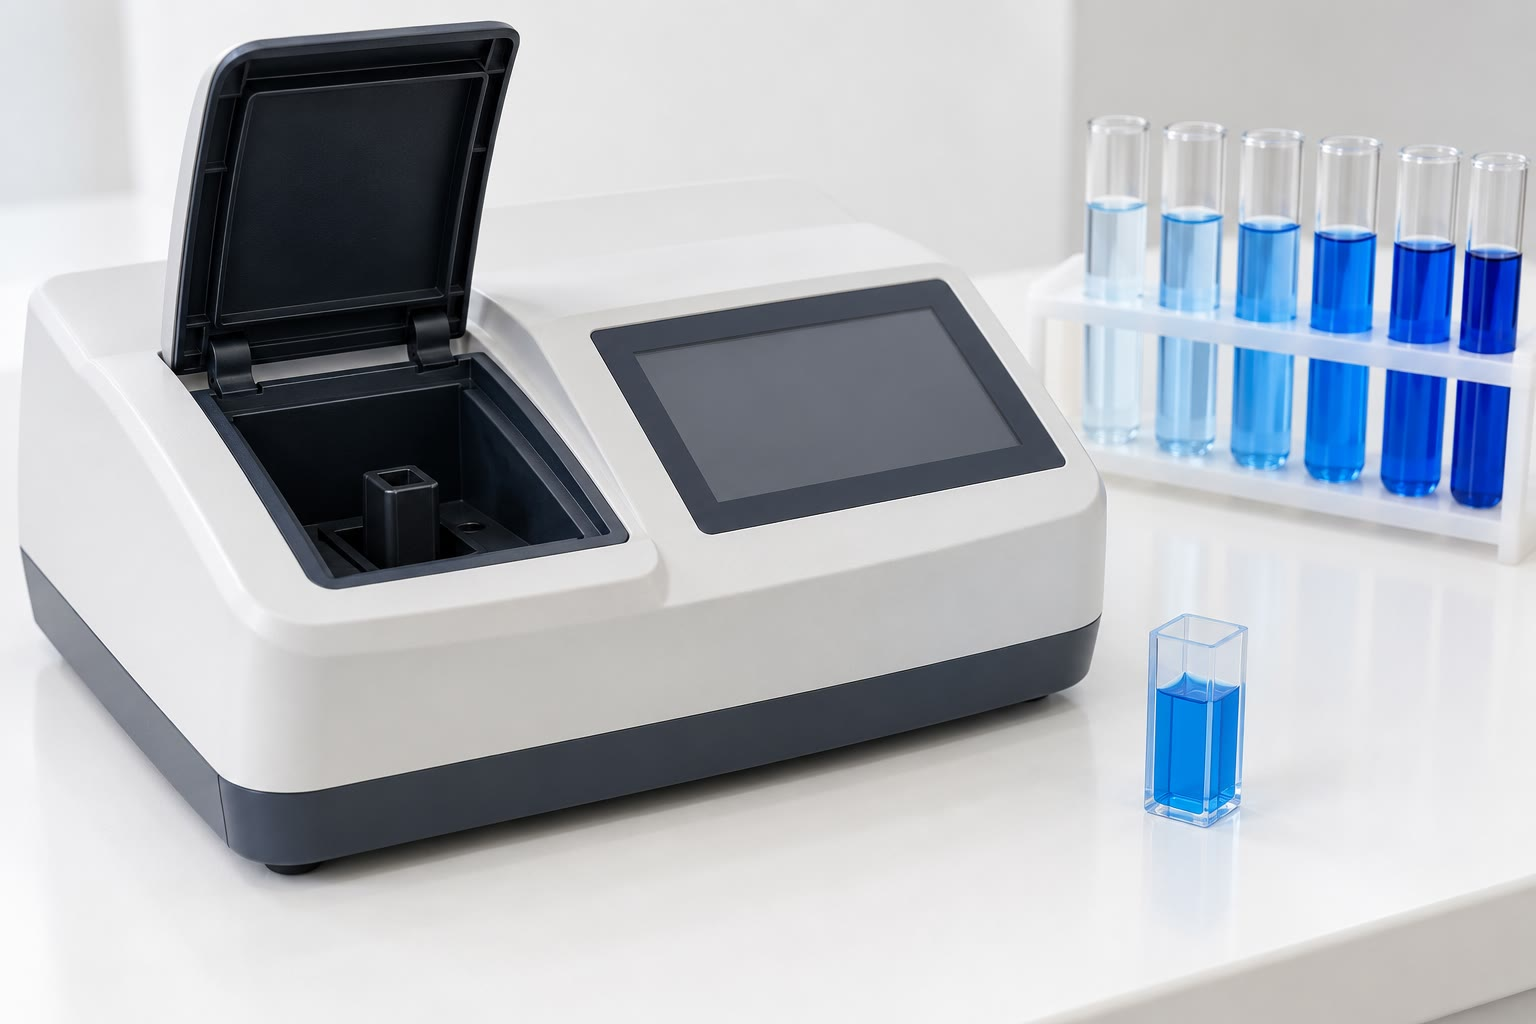
\includegraphics[width=0.5\linewidth]{images/book1/ai/g11-spectrophotometer.jpg}

{\small A spectrophotometer and its square cells.}
\end{omfigure}

\section{The Beer--Lambert law}

\begin{definition}[Molar absorption coefficient]\label{def:g11:absorbance:epsilon}
The \emph{molar absorption coefficient}\index{molar absorption coefficient}
$\varepsilon$ of a dissolved species, at a given
wavelength, measures how strongly one \omterm{def:g10:the-mole:amount}{mole} of it absorbs light; it
depends on the species, the \omterm{def:g6:solutions-and-solubility:solute}{solvent} and the wavelength, and is expressed
in \si{L/(mol.cm)}.
\end{definition}

\begin{proposition}[Beer--Lambert law]\label{prop:g11:absorbance:beer-lambert}
For a dilute solution of a single absorbing species, of \omterm{def:g10:concentration-and-dilution:molar-concentration}{molar
concentration} $c$, in a cell of thickness $\ell$, the \omterm{def:g11:absorbance:absorbance}{absorbance} at a
given wavelength is
\[
  A = \varepsilon\, \ell\, c .
\]
The \omterm{def:g11:absorbance:absorbance}{absorbance} is proportional to the concentration.
\end{proposition}

\begin{proof}
Admitted here; it is derived in a university volume.
\end{proof}


\begin{remark}[With a mass concentration]\label{rem:g11:absorbance:mass}
% ledger: abs:E133, mw:E133
Since $c = C_m / M$, the law can also be written $A = a\, \ell\, C_m$,
with $a = \varepsilon / M$ in \si{L/(g.cm)}. The specifications of food
dyes give $a$: for the blue dye E133 at \qty{629}{nm}, $a =
\qty{164}{L/(g.cm)}$, and with its \omterm{def:g10:the-mole:molar-mass}{molar mass} of \qty{792.9}{g/mol},
$\varepsilon = 164 \times 792.9 = \qty{1.30e5}{L/(mol.cm)}$. A solution
of only \qty{5.0}{mg/L} of it, in a \qty{1}{cm} cell, already reads
$A = 164 \times 1 \times 0.0050 = 0.82$.
\end{remark}

\begin{remark}[Dilute solutions only]\label{rem:g11:absorbance:dilute}
The proportionality holds only for dilute solutions, in practice for
\omterm{def:g11:absorbance:absorbance}{absorbances} below about 1 to 1.5 on an ordinary instrument. A solution
that is too concentrated is diluted by a known factor before it is
measured.
\end{remark}

\section{Measuring a concentration}

\begin{definition}[Calibration line]\label{def:g11:absorbance:calibration-line}
A \emph{calibration line}\index{calibration line} is the graph of the
\omterm{def:g11:absorbance:absorbance}{absorbance} of a series of \omterm{def:g10:concentration-and-dilution:standard}{standard solutions} of one species, measured at
the same wavelength in the same cell, against their concentration. When
the Beer--Lambert law holds, it is a straight line through the origin.
\end{definition}

\begin{method}[Measuring a concentration with a calibration line]\label{met:g11:absorbance:calibration}
\begin{enumerate}
  \item Record the \omterm{def:g11:absorbance:spectrum}{absorption spectrum} of the species and choose the
        wavelength $\lambda_{\max}$, where the \omterm{def:g11:absorbance:absorbance}{absorbance} is largest and
        varies least with a small error on the wavelength.
  \item Zero the instrument with the blank.
  \item Prepare \omterm{def:g10:concentration-and-dilution:standard}{standard solutions} by \omterm{def:g10:concentration-and-dilution:dilution}{dilution} of a \omterm{def:g10:concentration-and-dilution:dilution}{stock solution} and
        measure their \omterm{def:g11:absorbance:absorbance}{absorbances}.
  \item Plot $A$ against the concentration and draw the straight line
        through the origin closest to the points.
  \item Measure the unknown, diluted if needed so that its \omterm{def:g11:absorbance:absorbance}{absorbance}
        falls among those of the standards, and read its concentration
        on the line (or divide $A$ by the slope); multiply by the
        \omterm{def:g10:concentration-and-dilution:dilution}{dilution factor}.
\end{enumerate}
\end{method}

\begin{omfigure}
\begin{tikzpicture}
\begin{axis}[width=0.72\linewidth, height=6cm, xmin=0, xmax=5.6,
    ymin=0, ymax=0.95, xlabel={concentration of E133 (\si{mg/L})},
    ylabel={absorbance at \qty{629}{nm}}, axis lines*=left, ymajorgrids,
    xmajorgrids, grid style={gray!20}, tick label style={font=\small},
    label style={font=\small}]
  % ledger: abs:E133 (points synthetic: exact values + fixed offsets)
  \addplot[only marks, mark=*, mark size=2.2pt, omDef] table[x=C, y=A]
    {figdata/out/grade-11-absorbance-b.dat};
  \addplot[thick, omProp, domain=0:5.5] {0.164*x};
  \addplot[dashed, black!60] coordinates {(0,0.590) (3.6,0.590) (3.6,0)};
  \node[font=\small, anchor=south west] at (axis cs:0.1,0.6) {unknown: $A = 0.590$};
  \node[font=\small, anchor=west] at (axis cs:3.65,0.22) {\qty{3.6}{mg/L}};
\end{axis}
\end{tikzpicture}

{\small \omterm{def:g11:absorbance:calibration-line}{Calibration line} of the blue dye: five standards (points) and
the line through the origin, of slope \qty{0.164}{L/mg}. An unknown
reading $A = 0.590$ has a concentration of $0.590 / 0.164 =
\qty{3.6}{mg/L}$.}
\end{omfigure}

\begin{example}[The five standards]\label{ex:g11:absorbance:standards}
A \omterm{def:g10:concentration-and-dilution:dilution}{stock solution} of the blue dye at \qty{100}{mg/L} is diluted to give
\qty{100.0}{mL} of each standard: for \qty{2.0}{mg/L}, the \omterm{def:g10:concentration-and-dilution:dilution}{dilution
factor} is 50, so \qty{2.0}{mL} of stock are made up to \qty{100.0}{mL}.
The five standards, from 1 to \qty{5}{mg/L}, read 0.168, 0.325, 0.494,
0.652 and 0.823: within a few thousandths of $0.164 \times C$, the line
of the figure.
\end{example}

\section{Exercises}

\begin{exercise}[$\star$]\label{exo:g11:absorbance:1}
A solution absorbs mainly orange light. What colour does it look? And a
solution that absorbs mainly violet light?
\end{exercise}

\begin{exercise}[$\star$]\label{exo:g11:absorbance:2}
Using the colour wheel, give the colour mainly absorbed by a green
solution, and the range of wavelengths that colour covers.
\end{exercise}

\begin{exercise}[$\star$]\label{exo:g11:absorbance:3}
Read on the absorption spectra the wavelength $\lambda_{\max}$ of each
dye and its \omterm{def:g11:absorbance:absorbance}{absorbance} there.
\end{exercise}

\begin{exercise}[$\star$]\label{exo:g11:absorbance:4}
A dye solution at \qty{2.0}{mg/L} reads $A = 0.30$. What does a solution
of the same dye at \qty{6.0}{mg/L} read in the same cell, at the same
wavelength? And at \qty{1.0}{mg/L}?
\end{exercise}

\begin{exercise}[$\star$]\label{exo:g11:absorbance:5}
What is the blank of a spectrophotometer, and why is the instrument set
to zero with it?
\end{exercise}

\begin{exercise}[$\star\star$]\label{exo:g11:absorbance:6}
Using the \omterm{def:g11:absorbance:calibration-line}{calibration line} of the blue dye, find the concentration of a
solution that reads $A = 0.41$.
\end{exercise}

\begin{exercise}[$\star\star$]\label{exo:g11:absorbance:7}
To measure the blue dye, why set the spectrophotometer to
\qty{629}{nm} rather than to \qty{550}{nm}? Give two reasons.
\end{exercise}

\begin{exercise}[$\star\star$]\label{exo:g11:absorbance:8}
An undiluted drink reads $A = 2.4$ at \qty{629}{nm}, too high to be
trusted. It is diluted five times and then reads $A = 0.48$. Find the
concentration of blue dye in the drink.
\end{exercise}

\begin{exercise}[$\star\star$]\label{exo:g11:absorbance:9}
% ledger: mw:E102, abs:E102
A solution of tartrazine at \qty{15.0}{mg/L} reads $A = 0.795$ at
\qty{427}{nm} in a \qty{1.00}{cm} cell. Compute its absorptivity $a$ in
\si{L/(g.cm)}, then its \omterm{def:g11:absorbance:epsilon}{molar absorption coefficient} (\omterm{def:g10:the-mole:molar-mass}{molar mass}
\qty{534.4}{g/mol}).
\end{exercise}

\begin{exercise}[$\star\star$]\label{exo:g11:absorbance:10}
Look at the spectra of the two dyes. Above which wavelength does the
yellow dye absorb almost nothing? Why can the blue dye be measured at
\qty{629}{nm} even in a green drink that also contains the yellow dye?
\end{exercise}

\begin{exercise}[$\star\star$]\label{exo:g11:absorbance:11}
The same solution is measured in a cell \qty{2.0}{cm} thick instead of
\qty{1.0}{cm}. How does its \omterm{def:g11:absorbance:absorbance}{absorbance} change? Why?
\end{exercise}

\begin{exercise}[$\star\star\star$]\label{exo:g11:absorbance:12}
Standards of the blue dye at 5, 10, 20 and \qty{40}{mg/L} read 0.82, 1.62,
2.30 and 2.70. Compute $A / C$ for each. What do you notice? Which
standards may be used for a \omterm{def:g11:absorbance:calibration-line}{calibration line}, and what should be done
with an unknown that reads $2.5$?
\end{exercise}

\begin{exercise}[$\star\star\star$]\label{exo:g11:absorbance:13}
A green drink contains the blue dye and the yellow dye. In a
\qty{1.00}{cm} cell it reads $A = 0.574$ at \qty{629}{nm} and $A = 0.53$
at \qty{427}{nm}. At \qty{427}{nm} the blue dye absorbs almost nothing,
and at \qty{629}{nm} the yellow dye absorbs nothing. Find the \omterm{def:g10:concentration-and-dilution:mass-concentration}{mass
concentrations} of both dyes (use $a = \qty{164}{L/(g.cm)}$ and
$a = \qty{53.0}{L/(g.cm)}$).
\end{exercise}

\begin{exercise}[$\star\star\star$]\label{exo:g11:absorbance:14}
A student forgets the blank and sets the instrument to zero with an empty
cell. Every reading is then \num{0.040} too high. The unknown reads
$0.368$, and she divides by the slope $0.164$ of the true \omterm{def:g11:absorbance:calibration-line}{calibration
line}. What concentration does she find? What is the true one? By what
percentage is she wrong?
\end{exercise}

\begin{exercise}[$\star\star\star$]\label{exo:g11:absorbance:15}
% ledger: adi:E102
The acceptable daily intake of tartrazine is \qty{10}{mg} per kilogram
of body mass. A drink contains \qty{20}{mg/L} of it. What volume of the
drink would bring a \qty{60}{kg} adult to this intake in one day? Is
that a realistic risk?
\end{exercise}

\section{Problem: The Blue of a Sports Drink}


\begin{problem}[{Weekend problem --- how many bottles of a blue sports
drink would a child have to drink to reach the safe daily limit of its
dye?}]
\label{pb:g11:absorbance:1}
% ledger: lmax:E133, abs:E133, mw:E133, adi:E133
A food laboratory checks the blue dye E133 of a sports drink sold in
\qty{500}{mL} bottles. The specifications of the dye give its \omterm{def:g10:the-mole:molar-mass}{molar mass},
\qty{792.9}{g/mol}, and its acceptable daily intake: \qty{6}{mg} per
kilogram of body mass and per day, an amount that can be eaten every day
for a lifetime without appreciable risk.

\medskip
\noindent\textbf{Part I --- Colour and spectrum.}
\begin{enumerate}
  \item The drink looks blue. Using the colour wheel, which colour of
        light does it absorb most?
  \item Read the wavelength $\lambda_{\max}$ of the dye on its spectrum.
  \item Why is the \omterm{def:g11:absorbance:absorbance}{absorbance} of the dye almost zero at \qty{450}{nm}?
        Is that consistent with its colour?
  \item At which wavelength should the measurements be made?
\end{enumerate}

\medskip
\noindent\textbf{Part II --- The \omterm{def:g11:absorbance:calibration-line}{calibration line}.}
\begin{enumerate}[resume]
  \item \qty{50.0}{mg} of pure dye are dissolved to make \qty{500.0}{mL}
        of \omterm{def:g10:concentration-and-dilution:dilution}{stock solution}. Compute its \omterm{def:g10:concentration-and-dilution:mass-concentration}{mass concentration} in \si{mg/L}.
  \item Standards of 1.0, 2.0, 3.0, 4.0 and \qty{5.0}{mg/L} are made,
        \qty{100.0}{mL} each. What volume of stock is needed for the
        \qty{3.0}{mg/L} standard? With which glassware?
  \item The standards read 0.168, 0.325, 0.494, 0.652 and 0.823. Compute
        $A / C$ for each, and show that the points lie close to a line
        through the origin of slope about \qty{0.164}{L/mg}.
  \item Why must the line pass through the origin?
  \item Deduce the absorptivity $a$ of the dye in \si{L/(g.cm)} (cell of
        \qty{1.00}{cm}), then its \omterm{def:g11:absorbance:epsilon}{molar absorption coefficient}.
\end{enumerate}

\medskip
\noindent\textbf{Part III --- The drink.}
\begin{enumerate}[resume]
  \item \qty{25.0}{mL} of drink are made up to \qty{50.0}{mL} with water.
        What is the \omterm{def:g10:concentration-and-dilution:dilution}{dilution factor}?
  \item The diluted drink reads $A = 0.590$. Find its concentration of
        dye.
  \item Deduce the concentration of dye in the drink itself.
  \item What would the undiluted drink read? Why was it diluted?
  \item Compute the mass of dye in one bottle.
  \item Compute the amount of dye, in \omterm{def:g10:the-mole:amount}{moles}, in one bottle.
\end{enumerate}

\medskip
\noindent\textbf{Part IV --- The acceptable daily intake.}
\begin{enumerate}[resume]
  \item What mass of the dye may a child of \qty{30}{kg} take in each
        day?
  \item How many bottles would the child have to drink in one day to
        reach it?
  \item What volume of drink is that? Comment.
  \item Same question for an adult of \qty{70}{kg}.
  \item State the final answer: how many \qty{500}{mL} bottles would a
        \qty{30}{kg} child have to drink in a day to reach the
        acceptable daily intake of the dye?
\end{enumerate}
\end{problem}
